\documentclass[a4paper,UKenglish,cleveref, autoref, thm-restate]{lipics-v2021}
%This is a template for producing LIPIcs articles. 
%See lipics-v2021-authors-guidelines.pdf for further information.
%for A4 paper format use option "a4paper", for US-letter use option "letterpaper"
%for british hyphenation rules use option "UKenglish", for american hyphenation rules use option "USenglish"
%for section-numbered lemmas etc., use "numberwithinsect"
%for enabling cleveref support, use "cleveref"
%for enabling autoref support, use "autoref"
%for anonymousing the authors (e.g. for double-blind review), add "anonymous"
%for enabling thm-restate support, use "thm-restate"
%for enabling a two-column layout for the author/affilation part (only applicable for > 6 authors), use "authorcolumns"
%for producing a PDF according the PDF/A standard, add "pdfa"

%\pdfoutput=1 %uncomment to ensure pdflatex processing (mandatatory e.g. to submit to arXiv)
%\hideLIPIcs  %uncomment to remove references to LIPIcs series (logo, DOI, ...), e.g. when preparing a pre-final version to be uploaded to arXiv or another public repository

%\graphicspath{{./graphics/}}%helpful if your graphic files are in another directory

\bibliographystyle{plainurl}% the mandatory bibstyle

\title{On Piecewise Affine Reachability with Bellman Operators}

%\titlerunning{Dummy short title} %TODO optional, please use if title is longer than one line

%\author{Jane {Open Access}}{Dummy University Computing Laboratory, Country \and My second affiliation, Country \and \url{http://www.myhomepage.edu} }{johnqpublic@dummyuni.org}{https://orcid.org/0000-0002-1825-0097}{(Optional) author-specific funding acknowledgements}%TODO mandatory, please use full name; only 1 author per \author macro; first two parameters are mandatory, other parameters can be empty. Please provide at least the name of the affiliation and the country. The full address is optional. Use additional curly braces to indicate the correct name splitting when the last name consists of multiple name parts.

\author{Anton Varonka}{TU Wien, Austria}{anton.varonka@tuwien.ac.at}{https://orcid.org/0000-0001-5758-0657}{}
\author{Kazuki Watanabe}{National Institute of Informatics, Japan}{}{https://orcid.org/0000-0002-4167-3370}{}
\authorrunning{A.\ Varonka and K.\ Watanabe} 

\Copyright{Anton Varonka and Kazuki Watanabe}

\ccsdesc[500]{Theory of computation~Abstract machines}
\ccsdesc[500]{Mathematics of computing~Markov processes}
\ccsdesc[500]{Theory of computation~Program verification}

\keywords{piecewise affine map, reachability, value iteration, Markov decision process, Bellman operator}

\category{} %optional, e.g. invited paper

\relatedversion{} %optional, e.g. full version hosted on arXiv, HAL, or other respository/website
%\relatedversiondetails[linktext={opt. text shown instead of the URL}, cite=DBLP:books/mk/GrayR93]{Classification (e.g. Full Version, Extended Version, Previous Version}{URL to related version} %linktext and cite are optional

%\supplement{}%optional, e.g. related research data, source code, ... hosted on a repository like zenodo, figshare, GitHub, ...
%\supplementdetails[linktext={opt. text shown instead of the URL}, cite=DBLP:books/mk/GrayR93, subcategory={Description, Subcategory}, swhid={Software Heritage Identifier}]{General Classification (e.g. Software, Dataset, Model, ...)}{URL to related version} %linktext, cite, and subcategory are optional

%\funding{(Optional) general funding statement \dots}%optional, to capture a funding statement, which applies to all authors. Please enter author specific funding statements as fifth argument of the \author macro.

%\acknowledgements{The authors want to thank \dots}%optional

%\nolinenumbers %uncomment to disable line numbering

%
% --- inline annotations
%
\newcommand{\red}[1]{{\color{red}#1}}
\newcommand{\todo}[1]{{\color{red}#1}}
\newcommand{\TODO}[1]{\textbf{\color{red}[TODO: #1]}}
% --- disable by uncommenting  
% \renewcommand{\TODO}[1]{}
% \renewcommand{\todo}[1]{#1}



\newcommand{\VLM}{LVLM\xspace} 
\newcommand{\ours}{PeKit\xspace}
\newcommand{\yollava}{Yo’LLaVA\xspace}

\newcommand{\thisismy}{This-Is-My-Img\xspace}
\newcommand{\myparagraph}[1]{\noindent\textbf{#1}}
\newcommand{\vdoro}[1]{{\color[rgb]{0.4, 0.18, 0.78} {[V] #1}}}
% --- disable by uncommenting  
% \renewcommand{\TODO}[1]{}
% \renewcommand{\todo}[1]{#1}
\usepackage{slashbox}
% Vectors
\newcommand{\bB}{\mathcal{B}}
\newcommand{\bw}{\mathbf{w}}
\newcommand{\bs}{\mathbf{s}}
\newcommand{\bo}{\mathbf{o}}
\newcommand{\bn}{\mathbf{n}}
\newcommand{\bc}{\mathbf{c}}
\newcommand{\bp}{\mathbf{p}}
\newcommand{\bS}{\mathbf{S}}
\newcommand{\bk}{\mathbf{k}}
\newcommand{\bmu}{\boldsymbol{\mu}}
\newcommand{\bx}{\mathbf{x}}
\newcommand{\bg}{\mathbf{g}}
\newcommand{\be}{\mathbf{e}}
\newcommand{\bX}{\mathbf{X}}
\newcommand{\by}{\mathbf{y}}
\newcommand{\bv}{\mathbf{v}}
\newcommand{\bz}{\mathbf{z}}
\newcommand{\bq}{\mathbf{q}}
\newcommand{\bff}{\mathbf{f}}
\newcommand{\bu}{\mathbf{u}}
\newcommand{\bh}{\mathbf{h}}
\newcommand{\bb}{\mathbf{b}}

\newcommand{\rone}{\textcolor{green}{R1}}
\newcommand{\rtwo}{\textcolor{orange}{R2}}
\newcommand{\rthree}{\textcolor{red}{R3}}
\usepackage{amsmath}
%\usepackage{arydshln}
\DeclareMathOperator{\similarity}{sim}
\DeclareMathOperator{\AvgPool}{AvgPool}

\newcommand{\argmax}{\mathop{\mathrm{argmax}}}     


\nolinenumbers
\begin{document}

\maketitle

\begin{abstract}	
	A piecewise affine map is one of the simplest mathematical objects exhibiting complex dynamics.
	The reachability problem of piecewise affine maps is given as follows: Given two vectors $\bm{s}, \bm{t} \in \QQ^d$ and a piecewise affine map $f$, is there $n\in \NN$ such that $f^{n}(\bm{s}) = \bm{t}$?
	Koiran, Cosnard, and Garzon show that the reachability problem of piecewise affine maps is undecidable even in dimension~2. 
	
	Most of the recent progress has been focused on decision procedures for one-dimensional piecewise affine maps, 
	where the reachability problem has been shown to be decidable for some subclasses.
	However, the general undecidability
	discouraged research into positive results in arbitrary dimension.

	
	In this work, we consider a rich subclass of piecewise affine maps defined by Bellman operators of Markov decision processes (MDPs).
	We then investigate the restriction of the piecewise affine reachability problem to that with Bellman operators and, in particular, its decidability
	in any dimension.
	As one of our primary contributions,  we establish the decidability
	of reachability for two-dimensional Bellman operators, in contrast to the negative result known for general piecewise affine maps.
\end{abstract}

\section{Introduction}


\begin{figure}[t]
\centering
\includegraphics[width=0.6\columnwidth]{figures/evaluation_desiderata_V5.pdf}
\vspace{-0.5cm}
\caption{\systemName is a platform for conducting realistic evaluations of code LLMs, collecting human preferences of coding models with real users, real tasks, and in realistic environments, aimed at addressing the limitations of existing evaluations.
}
\label{fig:motivation}
\end{figure}

\begin{figure*}[t]
\centering
\includegraphics[width=\textwidth]{figures/system_design_v2.png}
\caption{We introduce \systemName, a VSCode extension to collect human preferences of code directly in a developer's IDE. \systemName enables developers to use code completions from various models. The system comprises a) the interface in the user's IDE which presents paired completions to users (left), b) a sampling strategy that picks model pairs to reduce latency (right, top), and c) a prompting scheme that allows diverse LLMs to perform code completions with high fidelity.
Users can select between the top completion (green box) using \texttt{tab} or the bottom completion (blue box) using \texttt{shift+tab}.}
\label{fig:overview}
\end{figure*}

As model capabilities improve, large language models (LLMs) are increasingly integrated into user environments and workflows.
For example, software developers code with AI in integrated developer environments (IDEs)~\citep{peng2023impact}, doctors rely on notes generated through ambient listening~\citep{oberst2024science}, and lawyers consider case evidence identified by electronic discovery systems~\citep{yang2024beyond}.
Increasing deployment of models in productivity tools demands evaluation that more closely reflects real-world circumstances~\citep{hutchinson2022evaluation, saxon2024benchmarks, kapoor2024ai}.
While newer benchmarks and live platforms incorporate human feedback to capture real-world usage, they almost exclusively focus on evaluating LLMs in chat conversations~\citep{zheng2023judging,dubois2023alpacafarm,chiang2024chatbot, kirk2024the}.
Model evaluation must move beyond chat-based interactions and into specialized user environments.



 

In this work, we focus on evaluating LLM-based coding assistants. 
Despite the popularity of these tools---millions of developers use Github Copilot~\citep{Copilot}---existing
evaluations of the coding capabilities of new models exhibit multiple limitations (Figure~\ref{fig:motivation}, bottom).
Traditional ML benchmarks evaluate LLM capabilities by measuring how well a model can complete static, interview-style coding tasks~\citep{chen2021evaluating,austin2021program,jain2024livecodebench, white2024livebench} and lack \emph{real users}. 
User studies recruit real users to evaluate the effectiveness of LLMs as coding assistants, but are often limited to simple programming tasks as opposed to \emph{real tasks}~\citep{vaithilingam2022expectation,ross2023programmer, mozannar2024realhumaneval}.
Recent efforts to collect human feedback such as Chatbot Arena~\citep{chiang2024chatbot} are still removed from a \emph{realistic environment}, resulting in users and data that deviate from typical software development processes.
We introduce \systemName to address these limitations (Figure~\ref{fig:motivation}, top), and we describe our three main contributions below.


\textbf{We deploy \systemName in-the-wild to collect human preferences on code.} 
\systemName is a Visual Studio Code extension, collecting preferences directly in a developer's IDE within their actual workflow (Figure~\ref{fig:overview}).
\systemName provides developers with code completions, akin to the type of support provided by Github Copilot~\citep{Copilot}. 
Over the past 3 months, \systemName has served over~\completions suggestions from 10 state-of-the-art LLMs, 
gathering \sampleCount~votes from \userCount~users.
To collect user preferences,
\systemName presents a novel interface that shows users paired code completions from two different LLMs, which are determined based on a sampling strategy that aims to 
mitigate latency while preserving coverage across model comparisons.
Additionally, we devise a prompting scheme that allows a diverse set of models to perform code completions with high fidelity.
See Section~\ref{sec:system} and Section~\ref{sec:deployment} for details about system design and deployment respectively.



\textbf{We construct a leaderboard of user preferences and find notable differences from existing static benchmarks and human preference leaderboards.}
In general, we observe that smaller models seem to overperform in static benchmarks compared to our leaderboard, while performance among larger models is mixed (Section~\ref{sec:leaderboard_calculation}).
We attribute these differences to the fact that \systemName is exposed to users and tasks that differ drastically from code evaluations in the past. 
Our data spans 103 programming languages and 24 natural languages as well as a variety of real-world applications and code structures, while static benchmarks tend to focus on a specific programming and natural language and task (e.g. coding competition problems).
Additionally, while all of \systemName interactions contain code contexts and the majority involve infilling tasks, a much smaller fraction of Chatbot Arena's coding tasks contain code context, with infilling tasks appearing even more rarely. 
We analyze our data in depth in Section~\ref{subsec:comparison}.



\textbf{We derive new insights into user preferences of code by analyzing \systemName's diverse and distinct data distribution.}
We compare user preferences across different stratifications of input data (e.g., common versus rare languages) and observe which affect observed preferences most (Section~\ref{sec:analysis}).
For example, while user preferences stay relatively consistent across various programming languages, they differ drastically between different task categories (e.g. frontend/backend versus algorithm design).
We also observe variations in user preference due to different features related to code structure 
(e.g., context length and completion patterns).
We open-source \systemName and release a curated subset of code contexts.
Altogether, our results highlight the necessity of model evaluation in realistic and domain-specific settings.






\section{Preliminaries}\label{sec:prelim}

We recall some definitions and properties for Bellman operators and Markov decision processes (MDPs), which are necessary for our development. 

\begin{definition}[MDP~\cite{Puterman94}]
    An MDP $\mdp$ is a tuple $(S, A, \prob)$ such that (i) $S$ is a finite non-empty set of \emph{states}; 
    (ii) $A$ is a finite non-empty set of \emph{actions}; and (iii) $\prob$ is the transition probability function~$\prob(s, \alpha, \_) \in S\rightarrow [0, 1]$ with finite support that satisfies $\sum_{s'\in S} \prob(s, \alpha, s') = 1$, for any $s\in S$ and $\alpha \in A$. 
\end{definition}

We refer to the support of $\prob(s, \alpha, \_)$ by $\supp(s, \alpha)$.
We fix a \emph{target state}~$t$ and assume that~$t$ is a sink, i.e.\ $\prob(t, \alpha, t) = 1$ for any $\alpha \in A$.
Given a state~$s \in S$,
a \emph{path} $\pi$ from $s$ to $t$ is a sequence $\pi \coloneqq (s_1,\dots, s_m)$ such that $s_i\in S\backslash \{t\} $ for any $i\in [1, m-1]$, $s_1 = s$, and $s_m  = t$.
We denote the set of paths from~$s$ to~$t$ by $\pathset{s}{t}$. 
%
A \emph{scheduler} is a function $\sigma\colon S^{+}\rightarrow A$.
As deterministic schedulers suffice for the reachability objective~\cite{bk}, we further consider
the set~$\Sigma$ of all deterministic schedulers. 
A scheduler is \emph{positional} if for any $s_1\cdots s_m\cdot s$ and $s'_1\cdots s'_n\cdot s$, the actions $\sigma(s_1\cdots s_m\cdot s)$ and 
$\sigma(s'_1\cdots s'_n\cdot s)$ coincide. 
For a path $\pi \coloneqq (s_1,\dots, s_m)$ and a scheduler $\sigma \in \Sigma$,
define $\prob^{\sigma}(\pi)\coloneqq \prod_{i\in [1, m-1]} \prob(s_i, \sigma(\pi_i), s_{i+1})$, where 
$\pi_i = (s_1,\dots, s_i)$.  

\begin{definition}[reachability probability]
    Given a scheduler $\sigma$, and $s\in S$, the \emph{reachability probability} $\prob^\sigma(s \models \lozenge t)$ under $\sigma$ is defined by 
    $\prob^\sigma(s \models \lozenge t)\coloneqq \sum_{\pi \in \pathset{s}{t}} \prob^{\sigma}(\pi)$. 
    
    The \emph{optimal reachability probability} is defined as $p_s:=\sup_{\sigma\in \Sigma} \prob^\sigma(s \models \lozenge t) $.
\end{definition}
We write~$\bm{p^*}$ for the vector $(p_s)_{s \in S\backslash \{t\}}$ indexed by states~$S\backslash \{t\}$.
The optimal reachability probabilities are in fact achievable by a positional scheduler. 
\begin{proposition}[e.g.~\cite{bk}] %[Lemma 10.102]
	\label{vi-positional}
    There exists an optimal positional scheduler~$\sigma_\text{pos} \in \Sigma$ such that
    $\prob^{\sigma_\text{pos}}(s \models \lozenge t) = p_s$ holds for all~$s \in S$.
\end{proposition}

\emph{Value Iteration (VI)}~\cite{bk,Puterman94} is a standard technique to approximate the vector of optimal reachability probabilities~$\bm{p^*}$. 
Specifically, VI applies the \emph{Bellman operator} $\Phi$ to the current approximation for each iteration step. 
\begin{definition}[Bellman operator]
    Let $S_d = \{s_1,\cdots, s_d\}$ be the set of all non-target states whose optimal reachability probability is positive.
    The \emph{Bellman operator} $\Phi \colon [0, 1]^d\rightarrow [0, 1]^d$ is defined by 
    \[
        \Phi(\bm{x})_s \coloneqq \max_{\alpha\in A} \sum_{s'\in S_d} \prob(s, \alpha, s') x_{s'}  + \prob(s, \alpha, t), 
    \] for each $\bm{x} = (x_s)_{s \in S_d}\in [0, 1]^d$ and $s\in S_d$.
\end{definition}
We note in passing that the set~$S_d$ can be computed using graph reachability techniques, see, e.g., \cite[Chapter 10.6.1]{bk}.
Given an appropriate initial vector $\bm{s}$, VI is then defined by the iteration $\langle\Phi^n(\bm{s})\rangle_{n \in \NN}$ that converges to the optimal reachability probabilities $\bm{p^*}$.

We further assume that the sets $Act_i$, $1 \leq i \leq d$, of actions available in state~$s_i \in S_d$ are disjoint.
Each action $\alpha \in Act_i$ is thus associated with a set $\suc(\alpha)$ of successor states defined as $\suc(\alpha):= \supp(s_i, \alpha) \cap S_d$. We emphasise that the successor set, together with transition probabilities~$\prob(s, \alpha, s')$, $s' \in S_d$, is a probabilistic \emph{sub}distribution.

We associate a polynomial of degree~1, \emph{a linear polynomial} of~$\alpha$, with each action $\alpha \in Act_i$. This polynomial $L_\alpha \in \QQ[\bm{x}]$ is defined as 
\[L_\alpha(\bm{x}) = \sum_{s' \in S_d} \prob(s_i, \alpha, s') x_{s'}  + \prob(s_i, \alpha, t).\]


For simplicity of notation, we might refer to states of~$S_d$ simply by their indices from~$\{1, \dots, d\}$ respectively denoting $\bm{x} = (x_1, \dots, x_d)$ and $\bm{p^*} = (p_1, \dots, p_d)$. 
Generally, vectors in this paper are typed in bold print.
We write $\bm{v} \geq \bm{0}$ ($\bm{v} > \bm{0}$) if every entry of~$\bm{v}$ is non-negative (resp.\ positive).
Furthermore, $\bm{u} \geq \bm{v}$ by definition holds if and only if $\bm{u} - \bm{v} \geq 0$; similarly for strict inequalities~$\bm{u} > \bm{v}$.
We refer to vectors~$\bm{u},\bm{v} \in \RR^d$ as \emph{comparable} if either $\bm{u} \geq \bm{v}$ or $\bm{u} \leq \bm{v}$ holds. 
Otherwise, the vectors are incomparable, denoted~$\bm{u} \bowtie \bm{v}$.

Let $||\cdot||_\infty$ denote the \emph{$\ell^\infty$-norm}, or the \emph{$\max$-norm}, defined by \(||\bm{x}||_\infty := \max{\left(|x_1|, \dots, |x_d|\right)}\) for a vector~$\bm{x} = (x_1, \dots, x_d) \in [0,1]^d$.
In the sequel, the notation $||\bm{x}||$ stands for $||\bm{x}||_\infty$.
We further define the $\ell^\infty$-metric, i.e., the distance between two vectors $\bm{x}$ and $\bm{y}$ is, respectively,
\(d(\bm{x},\bm{y}):= \max_i{\left(|x_i - y_i|\right)}.\)

Since the set $[0, 1]^d$ is a complete lattice with the pointwise ordering and the Bellman operator is monotone and $\omega$-continuous, the iterative update by the Bellman operator~$\Phi$ from the bottom vector~$\bm{0} \coloneqq (0, \cdots, 0)\in [0, 1]^d$ converges to the least fixed point~$\mu\Phi$, which is the optimal reachability probabilities $\bm{p^*} = (p_1,\cdots, p_d)$.

\begin{proposition}[\cite{bk,chatterjee2008vi,Puterman94}]
    The sequence $\langle\Phi^n(\mathbf{0})\rangle_{n\in \NN}$ is monotonically increasing and converges to the optimal reachability probabilities $\bm{p^*}$. 
\end{proposition}

By the Kleene fixed-point theorem, we can further see that the iteration by $\Phi$ converges to $\bm{p^*}$ from any initial values if $\Phi$ has a unique fixed point. 
In fact, the optimal reachability probabilities $\bm{p^*}$ are the unique fixed point $\mu\Phi$ when $\Phi$ has the unique fixed point. 
\begin{proposition}\label{all-converge}
    Assume $\Phi$ has a unique fixed point. 
    The sequence $\langle\Phi^n(\bm{x})\rangle_{n\in \NN}$ converges to $\bm{p^*}$ from any initial $\bm{x}\in [0, 1]^d$. 
\end{proposition}

In general, a Bellman operator has multiple fixed points, and there is a polynomial-time procedure to construct an equivalent MDP such that its Bellman operator has a unique fixed point; see~\cite{HaddadM18} for the details. 
In this paper, we assume that the Bellman operator has a unique fixed point, which can be ensured by the procedure in~\cite{HaddadM18}.  


\section{Bellman Operator Reachability in arbitrary dimension}
\label{sec:efs}
	
	We begin this section by recalling the value iteration algorithm.
	As an iterative procedure, Value Iteration boils down to repeatedly applying the Bellman operator~$\Phi$ starting from a certain vector~$\bm{s} \in [0,1]^d$ (usually, $\bm{s} = \bm{0}$) and converging to the unique fixed point~$\mu\Phi (= \bm{p^*})$.
	
	
	Now, observe that every Bellman operator~$\Phi$
	is indeed a piecewise affine map on the domain~$[0,1]^d$.
	On close inspection, for every~$\bm{x} \in [0,1]^d$, the value of $\Phi(\bm{x})$ is computed as a maximum of finitely many affine functions~$\phi_1, \dots, \phi_k : [0,1]^d \rightarrow [0,1]^d$ evaluated at~$\bm{x}$.
	Let~$P_i \subseteq [0,1]^d$ be the set of points~$\bm{x} \in [0,1]^d$, for which
	$\phi_i(\bm{x}) \geq \phi_j(\bm{x})$ for each $j \neq i$.
	Two observations are straightforward: 1) each~$P_i$ is defined by a conjunction of linear inequalities; 2) every~$\bm{x}$ belongs to at least one set~$P_i$.
	Moreover, $\Phi$ is a well-defined function,
	which can be observed from $\bm{x} \in P_i \cap P_j$ implying $\phi_i(\bm{x}) = \phi_j(\bm{x})$.
	Therefore, $\Phi$ is a PAM on~$[0,1]^d$.
	
	We further investigate the specialisation of the piecewise affine reachability problem to Bellman operators.
	To this end, we need to consider all possible $(\bm{s},\bm{t})$-pairs of $[0,1]^d$-vectors.

\textbf{Problem BOR (Bellman Operator Reachability).}
Given two vectors $\bm{s}, \bm{t} \in [0,1]^d$ and a Bellman operator~$\Phi: [0,1]^d \rightarrow [0,1]^d$ of some MDP,
does there exist~$n \in \NN$ such that $\Phi^n(\bm{s}) = \bm{t}?$

First, we show that BOR is decidable when $\bm{t}$ is not the unique fixed point $\mu\Phi$. 
\begin{lemma}\label{Phi-lip-like}
	Let $\Phi: [0, 1]^d\rightarrow [0, 1]^d$ be a Bellman operator with a unique fixed point $\mu\Phi$.
	Consider an arbitrary vector~$\bm{x} \in [0,1]^d$ and let
	$\delta:= ||\bm{x} - \mu\Phi||$.
	We have $||\Phi(\bm{x}) - \mu\Phi|| \leq \delta$.
\end{lemma}
\begin{proof}
	It holds $\bm{x} \leq \mu\Phi + \bm{\delta}$, where $\bm{\delta} := (\delta, \dots, \delta)$.
	For any action~$\alpha$ in state~$i$, we have
	\begin{align*}L_{\alpha} (\mu\Phi + \bm{\delta})={} 
	&\sum_{j \in S_d} \prob(i,\alpha, j) \cdot (\mu\Phi_j + \delta) + \prob(i, \alpha, t)\\
	={}&\sum_{j \in S_d} \prob(i,\alpha, j) \cdot \mu\Phi_j + \prob(i, \alpha, t) + \sum_{j \in S_d} \prob(i,\alpha, j) \cdot \delta   \\
	={}&L_{\alpha}(\mu\Phi) +  \sum_{j \in S_d} \prob(i,\alpha, j) \cdot \delta \leq 
	L_{\alpha}(\mu\Phi) + \delta.
	\end{align*}
	Hence, $\Phi(\mu\Phi + \bm{\delta})_i = \max_{\alpha \in Act_i} L_\alpha(\mu\Phi + \bm{\delta})
	\leq L_\alpha(\mu\Phi) + \delta \leq \mu\Phi_i + \delta$.
	
	From monotonicity of~$\Phi$ we conclude $\Phi(\bm{x})_i \leq \Phi(\mu\Phi + \bm{\delta})_i \leq \mu\Phi_i + \delta$.
\end{proof}

\begin{proposition}\label{t-not-fp}
	Let~$\mathcal{M}$ be an MDP whose Bellman operator $\Phi: [0, 1]^d\rightarrow [0, 1]^d$ has a unique fixed point $\mu\Phi$.
	Let $\bm{s} \in [0,1]^d$ be an arbitrary initial vector.
	For every $\bm{t} \in [0,1]^d$ with $\bm{t} \neq \mu\Phi$, 
	there exists an effectively computable bound~$N$ such that
	\[\Phi^n(\bm{s}) = \bm{t} \quad \Rightarrow \quad \Phi^n(\bm{s}) = \bm{t} \text{ for some } n\leq N.\]
\end{proposition}
\begin{proof}
	Fix arbitrary vectors~$\bm{s}, \bm{t} \in [0,1]^d$ assuming $\bm{t} \neq \mu\Phi$.
	We crucially use the convergence properties of the interval iteration algorithm~\cite{HaddadM18}.
	Let $\bm{1}:= (1, \dots, 1)$ be the greatest element of the lattice~$[0, 1]^d$. 
	Choose a convergence threshold~$\varepsilon > 0$.
	From \cite[Theorem~2]{HaddadM18} we have $||\Phi^N(\bm{0}) - \Phi^N(\bm{1})|| < \varepsilon$ for some $N \leq A \lceil \frac{\log{\varepsilon}}{\log(1-B^A)} \rceil$,
	where constants~$A, B$ only depend on~$\mathcal{M}$ and can be computed directly from its representation.
	
	From the monotonicity of $\Phi$ we have $\Phi^N(\bm{0}) \leq \Phi^N(\bm{s}) \leq \Phi^N(\bm{1})$ for any~$\bm{s} \in [0,1]^d$.
	We also have $\Phi^N(\bm{0}) \leq \mu\Phi \leq \Phi^N(\bm{1})$, 
	and so 
	$||\Phi^N(\bm{s}) - \mu\Phi|| < \varepsilon$.

	Recall that we can compute the vector~$\mu\Phi$ exactly.
	Now choose the threshold $\varepsilon := ||\bm{t} - \mu\Phi||$, and let $N_\varepsilon$ be the previously discussed bound for this threshold.
	We have $||\Phi^{N_\varepsilon}(\bm{s}) - \mu\Phi|| <  ||\bm{t} - \mu\Phi||$  and hence,
	from~\cref{Phi-lip-like},
	 $||\Phi^n(\bm{s}) - \mu\Phi|| <  ||\bm{t} - \mu\Phi||$ for every~$n \geq N_\varepsilon$.
	Therefore, either $\bm{t} = \Phi^n(\bm{s})$ for some $n < N_\varepsilon$, or $\bm{t}$ is not reachable from $\bm{s}$ under iteratively applying~$\Phi$.
	The first condition can be checked in finite time 
	since $N_{\varepsilon}$ is effectively bounded.
\end{proof}

From \cref{t-not-fp} we immediately derive an algorithmic procedure for the BOR problem instances $(\Phi, \bm{s}, \bm{t})$, where $\bm{t} \neq \mu\Phi$. 
For an instance like this, it suffices to compute the bound~$N$ as above, and to test whether any~$n\leq N$ is equal to $\bm{t}$.

We now move on to the case $\bm{t} = \mu\Phi$.
In the sequel, it will be important to differentiate between two types of actions. These types are defined based on preserving the probabilities of the unique fixed point~$\bm{t} = (t_1, \dots, t_d)$.
\begin{definition}
	An action $\alpha$ available in state~$i$ is \emph{tight}, if $t_i = L_\alpha(t_1, \dots, t_d)$, where $L_\alpha$ is the linear polynomial of action $\alpha$.
	An action $\alpha$ is \emph{leaking} in state $i$, if it is not tight.
\end{definition}
%%%
\subsection{Initial vector below the fixed point.} \label{sec:below}
We now assume that $\bm{s} \leq \bm{t}$. 
Recall that $\bm{t}$ is the unique fixed point $\mu \Phi$ of~$\Phi$ and that the Bellman operator is monotone. 
In particular, $\Phi^n(\bm{s}) \leq \bm{t}$ holds for all $n \geq 0$.

\begin{lemma}\label{below-only-opt-succ}
	Let~$\bm{x} \leq \bm{t}$ be a $[0,1]^d$-vector 
	and let~$\alpha \in Act_i$ be the action chosen in state~$i$ when the Bellman operator is applied in~$\bm{x}$, 
	i.e.
	\(\Phi(\bm{x})_i = L_{\alpha}(\bm{x}).\)

	$\Phi(\bm{x})_i = t_i$ holds if and only if $\alpha$ is tight and for each~$j \in \suc(\alpha)$ we have $x_j = t_j$.
\end{lemma}
\begin{proof}
	One implication follows from directly applying the definitions.
	Now consider the ($\Rightarrow$) implication.
	For every action~$\beta$, we have $L_\beta(\bm{x}) \leq L_\beta(\bm{t})$.
	Hence, for a leaking~$\beta$, this implies $L_\beta(\bm{x}) < t_i$. 
	Since for~$\alpha$ we have $L_\alpha(\bm{x}) = t_i$, it must be tight.
	Assume further that there exists~$j \in \suc(\alpha)$ such that $x_j < t_j$. Then, $L_{\alpha}(\bm{x}) \leq L_{\alpha}(t_1, \dots, t_{j-1}, x_j, t_{j+1}, \dots, t_d) < L_{\alpha}(\bm{t}) = t_i$.
	This again contradicts $L_\alpha(\bm{x}) = t_i$, hence $x_j = t_j$ holds for all~$j \in \suc(\alpha)$.
\end{proof}

\subparagraph*{From probabilities to $\{-1,0\}$.} The reasoning of \cref{below-only-opt-succ} can be extended.
Intuitively, we can abstract away from the actual probabilities in vectors $\Phi^n(\bm{s})$, $n \geq 0$. This succeeds by \emph{only keeping track of whether these probabilities are different from probabilities in~$\bm{t}$}.
This abstraction makes the space of the BOR problem finite, provided $\bm{s} \leq \mu\Phi$.

Formally, we introduce a sign abstraction~$f: [0,1]^d \rightarrow \{-1, 0\}^d$ by associating a sign vector~$\eps = f(\bm{x}) = (\varepsilon_1, \dots, \varepsilon_d)$ with every vector~$\bm{x}$ such that $\bm{x} \le \bm{t}$:
\(\varepsilon_i = \begin{cases}
	0, & x_i = t_i,\\
	-1, & \text{otherwise}.
\end{cases}\)
According to this definition, $f(\bm{t}) = \bm{0}$.
\cref{below-only-opt-succ} can now be read as follows:
 $\Phi(\bm{x}) = \bm{t}$ holds if and only if 
 there exists a choice of tight actions~$(\alpha_1, \dots, \alpha_d)$ in~$\bm{x}$ (whose sign vector is~$\eps$) 
 such that for each state $s \in \suc{\alpha_i}$, we have $\varepsilon_s = 0$.
	
We further prove that the successor of $f(\bm{x})$ with respect to the Bellman operator is well-defined.
This would allow to only consider the evolution of sign vectors later on.
\begin{lemma}\label{abstr-below}
	Let~$\bm{x}$ and $\bm{y}$ be two vectors satisfying $\bm{x} \leq \bm{t}$ and $\bm{y} \leq \bm{t}$. 
	Provided $f(\bm{x}) = f(\bm{y})$, we have
	\(f(\Phi(\bm{x})) = f(\Phi(\bm{y})).\)
\end{lemma}
\begin{proof}
Let $\eps' = (\varepsilon'_1, \dots, \varepsilon'_d)$ be the abstraction of~$\Phi(\bm{x})$, that is, $\eps' = f(\Phi(\bm{x}))$.

First, notice that a leaking action chosen in state~$i$ always implies $L_\alpha(\cdot) < t_i$.
Second, recall that having $j \in \suc(\alpha)$ with $\cdot_j < t_j$ implies $L_\alpha(\cdot) < t_i$.
Hence, $\Phi(\cdot)_i = t_i$ if and only if there exists an action~$\alpha \in Act_i$ such that $L_\alpha(\cdot) = t_i$. 
This action is necessarily tight.
Using the vocabulary of the sign abstraction, we state
$f(\Phi(\cdot))_i = 0$ holds if and only if there exists a tight action~$\alpha \in Act_i$ such that $L_\alpha(\cdot) = t_i$.
We summarise these observations as 
\begin{equation}\label{phi-below}
	\epsilon'_i = \max_{\substack{\alpha \in Act_i \\ \alpha \text{ tight}}} \; \min_{j \in \suc(\alpha)} \epsilon_j,
\end{equation}
and thus make sure that $\varepsilon'_i$ does not depend on the actual values in~$\bm{x}$ and $\bm{y}$, as soon as those two vectors have the same sign abstraction.
\end{proof}

\begin{proposition}\label{below-decid}
	There exists an algorithmic procedure for the BOR problem instances $(\Phi, \bm{s}, \bm{t})$, where $\bm{s} \leq \mu\Phi$ and $\bm{t} = \mu\Phi$. 
\end{proposition}
\begin{proof}
	It suffices to observe that the reachability problem in~$\{-1,0\}^d$ is decidable.
	Given~$\bm{s}$, we compute its abstraction~$f(\bm{s})$ and ask whether $\bm{0}$ is reached by iteratively applying the map $\eps \mapsto \eps'$ as defined by~\cref{phi-below}.
	Once an already explored vector occurs in the sequence $\langle\eps = f(\bm{s}), \eps', \eps'', \dots \rangle$, 
	we can stop.
	This happens in at most~$2^d -1$ iterations.
	In this finite sequence, $\bm{0}$ occurs if and only if~$\bm{t}$ is reached by iterating~$\Phi$ starting from~$\bm{s}$.
	This is due to~\cref{abstr-below}.
\end{proof}
%%%
\subsection{Initial vector above the fixed point.} \label{sec:above}
Next assumption we are going to work with is $\bm{s} \geq \bm{t} = \mu \Phi$.
In this subsection, we prove~\cref{above-decid}, an analogue of~\cref{below-decid}.
However, as the following proofs witness, the case when~$\bm{s}$ is \emph{above} the fixed point~$\bm{t}$ is more intricate.
\begin{proposition}
	\label{above-decid}
	There exists an algorithmic procedure for the BOR problem instances $(\Phi, \bm{s}, \bm{t})$, where $\bm{s} \geq \mu\Phi$ and $\bm{t} = \mu\Phi$. 
\end{proposition}
%%
A new phenomenon occurs for sequences initialised with~$\bm{s} \geq \bm{t}$.
An iteration of the Bellman operator can choose a leaking action~$\beta \in Act_i$ over all tight actions available in state~$s_i$.
Intuitively, this happens if the successor states~$\suc(\beta)$ have probabilities significantly greater than optimal--enough to compensate for the ``leakage''~$t_i - L_\beta(\bm{t})$.
In other words, $\Phi(\bm{x})_i > L_{\alpha}(\bm{x})$ might hold for all tight~$\alpha \in Act_i$, 
unlike in the case $\bm{x} \leq \bm{t}$, cf.\ \cref{below-only-opt-succ}.
%%
\begin{figure}[t]
	\begin{minipage}[b]{0.33\columnwidth}
	\begin{center}
		\begin{tikzpicture}[on grid,auto]
			\node[state] (s0) {$\mathstrut s_1$};
			\node[dot] (n0) [below right=0.4 and 1 of s0] {};
			\node[state] (s1) [below right=0 and 1.5 of s0] {$\mathstrut s_2$};
			\node[state] (s2) [below right=0 and 1.5 of s1] {$\mathstrut s_3$};
			\node[state, accepting] (sp) [below left =1.25 and 0 of s1] {$t$};
			\node[] (me) [above left=0.5 and 0.5 of s0] {\small$\mdp_1$:};
			\path[->]
			(s0) edge [bend left] node[pos=0.5,inner sep=1pt] {$\beta$, 1/2} (s1)
			(s0) edge [bend right] node[swap,pos=0.7,inner sep=2pt] {$\alpha$} (n0)
			(n0) edge [bend right] node[pos=0.7,inner sep=1pt] {1/2} (sp)
			(s0) edge [bend right] node[swap,inner sep=1pt] {$\beta$, 5/12} (sp)
			(n0) edge [bend right] node[pos=0.6,inner sep=1pt] {1/3} (s2)
			(s1) edge [bend left] node[pos=0.5,inner sep=1pt] {1} (s2)
			(s2) edge [bend left] node[pos=0.5,inner sep=1pt] {1/4} (sp)
			;
		\end{tikzpicture}
	\end{center}
	\caption{An MDP $\mdp_1$.}
	\label{fig:mdpLeakingAbove}
	\end{minipage}
	\hfill
	\begin{minipage}[b]{0.5\columnwidth}
		\begin{center}
			\begin{tikzpicture}[on grid,auto]
				\node[state] (s1) {$\mathstrut s_1$};
				\node[dot] (n1) [above right= 0 and 1 of s1] {};
				\node[dot] (n2) [above right= 0 and -1 of s1] {};
				\node[state] (s2) [above right = 1 and 2 of s1] {$\mathstrut s_2$};
				\node[state] (s3) [above right = -1 and 2 of s1] {$\mathstrut s_3$};
				\node[state, accepting] (s4) [above right = -1 and 1 of s2] {$\mathstrut t$};
				\node[] (me) [above left=1 and 2.5 of n1] {\small$\mdp_2$:};
				\path[->]
				(s1) edge [bend right] node[swap,pos=0.4,inner sep=1pt] {$\alpha_1$} (n1)
				(s1) edge [bend right] node[swap,pos=0.4,inner sep=1pt] {$\alpha_2$} (n2)
				(n1) edge [bend right] node[swap,pos=0.6,inner sep=1pt] {1/3} (s1)
				(n2) edge [bend right] node[swap,pos=0.6,inner sep=1pt] {1/2} (s1)
				(n1) edge [bend right] node[pos=0.6,inner sep=1pt] {1/3} (s2)
				(n1) edge [bend left] node[swap,pos=0.6,inner sep=1pt] {1/3} (s3)
				(n2) edge [out = 85, in = 140] node[pos=0.6,inner sep=1pt] {1/4} (s2)
				(n2) edge [out = 275, in = 220] node[swap,pos=0.6,inner sep=1pt] {1/4} (s3)
				(s2) edge [bend left] node[pos=0.6,inner sep=1pt] {$\beta$, 1/6} (s4)
				(s3) edge [bend right] node[swap,pos=0.5,inner sep=1pt] {$\gamma$, 1/6} (s4)
				(s2) edge [bend right] node[swap,pos=0.6,inner sep=1pt] {$\beta$, 1/3} (s1)
				(s3) edge [bend left] node[pos=0.6,inner sep=1pt] {$\gamma$, 1/3} (s1)
				(s2) edge [loop,out=60,in=-0,looseness=4] node {$\beta$, 1/3} (s2)
				(s3) edge [loop,out=0,in=-60,looseness=4] node {$\gamma$, 1/3} (s3)
				;
			\end{tikzpicture}
		\caption{An MDP $\mdp_2$.}
		\label{fig:mdpNonPositional}
		\end{center}
		\end{minipage}
\end{figure}
\begin{example}
	Consider an MDP $\mdp_1$ in~\cref{fig:mdpLeakingAbove}. 
	It has~$S = \{s_1, s_2, s_3, s_4, t\}$ where the ``missing'' probabilistic transitions lead to~$s_4$.
	Moreover, $Act_4$ comprises a single action with $\prob(s_4, \cdot, s_4) = 1$.
	We omit~$s_4$ and transitions to/from it, for simplicity of presentation.
	
	There is one tight action $\alpha$ and one leaking action $\beta$ in~$s_1$.
	Let $\bm{s} \coloneq (1, 1/3, 2/3)$. Clearly, $\bm{s} > \mu\Phi = (7/12, 1/4, 1/4)$. 
	The tight action $\alpha$ is chosen for the first iteration, and $\Phi(\bm{s}) = \left(13/18, 2/3, 1/4\right)$. 
	Next, the leaking action $\beta$ is chosen and $\Phi^{2}(\bm{s}) = \left(9/12, 1/4, 1/4\right)$, and finally $\Phi^{3}(\bm{s}) = \bm{t}$ by choosing the tight action $\alpha$.
\end{example}

\subparagraph*{Only tight actions eventually.} 
However, we show that in a convergent sequence, the actions chosen by the Bellman operator~$\Phi$ are all tight, after some number of iterations.

\begin{lemma}\label{nbhd-tight}
	Let~$\mathcal{M}$ be an MDP whose Bellman operator $\Phi: [0, 1]^d\rightarrow [0, 1]^d$ has a unique fixed point $\mu\Phi = \bm{t}$.
	There exists a $\delta$-neighbourhood of the fixed point
	\[U_\delta(\bm{t}) = \{\bm{x} \in [0,1]^d : d(\bm{x}, \bm{t}) < \delta \}\]
	such that 
	for every $\bm{x} \in U_\delta(\bm{t})$, the vector $\Phi(\bm{x})$ is obtained by applying only tight actions.
	That is, 
	\[\Phi(\bm{x}) = \left(L_{\alpha_1}(\bm{x}), \dots, L_{\alpha_d}(\bm{x})\right),\]
	where each $\alpha_i \in Act_i$, $1\leq i\leq d$, is tight.
\end{lemma}
\begin{proof}
	
Since the transition probabilities in~$\mathcal{M}$ are rational numbers, one argues that $t_1, \dots, t_d$ are rational, too.
We consider the set of rational numbers that consists of
$t_1, \dots, t_d$, along with $L_\alpha(\bm{t})$ for each action~$\alpha$.
It is sufficient to consider leaking actions, by definition.
Let~$D$ be the least common denominator of the numbers in the aforedescribed set.


Let $\delta:= \frac{1}{2D}$ and pick~$\bm{x} \in U_\delta(\bm{t})$.
Further let $A = (\alpha_1, \dots, \alpha_d)$ be the actions chosen at~$\bm{x}$ by the Bellman operator~$\Phi$.
We show that each action in~$A$ is tight.
Denote by~$f_A$ the effect of applying~$A$, in particular:
\[f_A(\bm{t}) = \left(L_{\alpha_1} (\bm{t}), \dots, L_{\alpha_d} (\bm{t})\right) \quad \text{and} \quad
f_A(\bm{x}) = \Phi(\bm{x}).
\]

We notice that~$f_A$ is 1-Lipschitz (which, in fact, holds for any choice~$A$ of actions). 
Indeed, let us consider arbitrary~$\bm{u}, \bm{v} \in [0,1]^d$. 
We have \begin{align*}
	||f_A(\bm{u}) - f_A(\bm{v})|| &= \max_{1 \leq i \leq d} |L_{\alpha_i}(\bm{u}) - L_{\alpha_i}(\bm{v})|\\
&\leq\max_{1\leq i \leq d} \sum_{j \in \suc(\alpha_i)} \prob(i, \alpha_i, j)\cdot  \left| u_j-v_j \right|\\
&\leq \max_{1\leq i \leq d} \left(1 \cdot \max_{j \in \suc{\alpha_i}}|u_j - v_j|\right)=
\max_{1\leq i \leq d} \left| u_i-v_i \right| = ||\bm{u} - \bm{v}||.
\end{align*}
Utilising the 1-Lipschitz property, we observe $||f_A(\bm{t}) - \Phi(\bm{x})|| \leq ||\bm{t} - \bm{x}||$.
Moreover, we have $||\Phi(\bm{x}) - \bm{t}|| \leq ||\bm{x} - \bm{t}||$ due to~\cref{Phi-lip-like}.
Therefore, 
\begin{equation} \label{eq:A-optimal}
	||f_A(\bm{t}) - \bm{t}|| \leq ||f_A(\bm{t}) - \Phi(\bm{x})|| + ||\Phi(\bm{x}) - \bm{t}||
	\leq ||\bm{t} - \bm{x}|| + ||\bm{x} - \bm{t}|| < \delta + \delta = \frac{1}{D}. 
\end{equation} 

On the other hand, \[
||f_A(\bm{t}) - \bm{t}|| = \max_{1 \leq i \leq d} |L_{\alpha_i}(\bm{t}) - t_i|.
\]
By the definition of~$D$, we know that $L_{\alpha_i}(\bm{t}) \neq t_i$ implies $|L_{\alpha_i}(\bm{t}) - t_i| \geq \frac{1}{D}$.
We conclude from \cref{eq:A-optimal} that $f_A(\bm{t}) = \bm{t}$.
Equivalently, all actions chosen at~$\bm{x}$ are tight.
\end{proof}

The vector sequence $\bm{s}, \Phi(\bm{s}), \Phi^2(\bm{s}), \dots$ converges to~$\bm{t}$ due to~\cref{all-converge}. Therefore, it reaches a $\frac{1}{2D}$-neighbourhood of~$\bm{t}$ after finitely many steps.
Furthermore, an upper bound on the number of necessary steps can be computed as in~\cref{t-not-fp}.
\begin{corollary}\label{event-tight}
	Let~$\mathcal{M}$ be an MDP whose Bellman operator $\Phi: [0, 1]^d\rightarrow [0, 1]^d$ has a unique fixed point $\mu\Phi$.
	For an arbitrary initial vector $\bm{s} \in [0,1]^d$, there exists an effectively computable~$N \in \NN$ such that in the sequence
	\[\bm{s}, \Phi(\bm{s}), \Phi^2(\bm{s}), \dots\]
	for every $n \geq N$, $\Phi^{n+1}(\bm{s})$ is obtained by applying only tight actions to $\Phi^n(\bm{s})$.
\end{corollary}
We point out that the argument used in the proof of~\cref{nbhd-tight},
bears resemblance to (and is inspired by) the proof of~\cite[Theorem~3]{HaddadM18}.
However, the eventual optimality of tight actions,
which we establish here,
is not a matter of discussion in~\cite{HaddadM18} or any other work we know.

\subparagraph*{From probabilities to $\{0,1\}$.} We now extend the sign abstraction
from the previous section to encompass vectors above~$\bm{t}$.
Let~$f: [0,1]^d \rightarrow \{0,1\}^d$
be defined by associating a sign vector~$\eps = f(\bm{x}) = (\varepsilon_1, \dots, \varepsilon_d)$ with each vector~$\bm{x} \geq \bm{t}$:
\(\varepsilon_i = \begin{cases}
	0, & x_i = t_i,\\
	1, & \text{otherwise}.
\end{cases}\)

Conforming to this definition is $f(\bm{t}) = \bm{0}$.
As before, we show that~$f$ is well-defined.
\begin{lemma}\label{abstr-above}
	Let~$\delta$ be chosen as above
	to guarantee that~$\Phi$ only picks tight actions in the neighbourhood~$U_\delta(\bm{t})$.
	Consider vectors~$\bm{x},\bm{y} \in [0,1]^d$ satisfying 
	\(\bm{t} \; \leq \bm{x}, \bm{y} \leq \; \bm{t} + \left(\delta, \dots, \delta\right).\)
	
	Provided $f(\bm{x}) = f(\bm{y})$, we have
	\(f(\Phi(\bm{x})) = f(\Phi(\bm{y})).\)
\end{lemma}
\begin{proof}
	The assumption~$\bm{x}, \bm{y} \in U_{\frac{1}{2D}}(\bm{t})$ is necessary to shake off the effect of the leaking actions (cf.\ the assumptions of~\cref{abstr-below}).
	This way we guarantee that for every~$i$, there is a tight action~$\alpha \in Act_i$ with 
	$\Phi(\cdot)_i = L_\alpha(\cdot)$.
	It is not hard to see now that
	having $j \in \suc(\alpha)$ with $\cdot_j > t_j$ implies $L_\alpha(\cdot) > t_i$.
	Therefore, $\Phi(\cdot)_i = t_i$ if and only if there exists no tight action~$\alpha \in Act_i$ that depends on
	$j \in \suc(\alpha)$ with $\cdot_j > t_j$.
	Equivalently, we have
	\begin{equation}\label{phi-above}
		\epsilon'_i = \max_{\substack{\alpha \in Act_i \\ \alpha \text{ tight}}} \; \max_{j \in \suc(\alpha)} \epsilon_j,
	\end{equation}
where~$\eps' = (\varepsilon'_1, \dots, \varepsilon'_d)$ is the abstraction of~$\Phi(\bm{x})$, that is, $\eps' = f(\Phi(\bm{x}))$.

Therefore, the abstraction vectors of~$\Phi(\bm{x})$ and~$\Phi(\bm{y})$ do not depend on the actual values in~$\bm{x}$ and~$\bm{y}$, but only on its abstractions $f(\bm{x}) = f(\bm{y})$.
\end{proof}
The abstraction~$f$ is thus well-defined for vectors in a certain neighbourhood of~$\bm{t}$. 
\begin{proof}[Proof of~\cref{above-decid}]
	Starting at~$\bm{s}$ above the fixed point, $\bm{s} \geq \bm{t}$, we first compute the bound~$N$ of~\cref{event-tight}.
	If $\Phi^n(\bm{s}) = \bm{t}$ holds for some $n < N$, we terminate with a positive answer to the BOR problem.
	Otherwise, we continue with the abstraction argument.
	We compute~$f(\Phi^N(\bm{s}))$ and ask whether $\bm{0}$ is reached by iteratively applying the map $\eps \mapsto \eps'$ as defined by~\cref{phi-above}.
In at most~$2^d - 1$ iterations we either reach~$\bm{0}$,
or discover an ever-repeating vector subsequence that does not contain~$\bm{0}$.
The rest follows from~\cref{abstr-above}.
\end{proof}
Combining \cref{below-decid,above-decid}
, we obtain the following theorem.
\begin{theorem}\label{compar-decid}
	There exists an algorithmic procedure that solves all BOR problem instances $(\Phi, \bm{s}, \bm{t})$ with~$\bm{t} = \mu\Phi$ and
	\(\bm{s} \; \{\leq, \geq\} \; \mu\Phi.\)
\end{theorem}
\subsection{Initial and target vectors are incomparable.}
\label{sec:incomp}
We keep assuming~$\bm{t}= \mu\Phi$ and consider the remaining case, that is, the case when $\bm{s}$ and $\bm{t}$ are two incomparable vectors,
denoted $\bm{s} \bowtie \bm{t}$.

We can assume $\bm{s} \in U_\delta(\bm{t})$ as defined in~\cref{nbhd-tight}.
Clearly, starting with an arbitrary incomparable vector, we can apply~$\Phi$ up to the pre-computed power~$N$,
reaching either a comparable vector (potentially including~$\bm{t}$ itself), or the $\delta$-neighbourhood of~$\bm{t}$.
In the latter case, set $\bm{s}$ to be the first vector inside the neighbourhood.
Hence, for every $\bm{x}$ discussed below, the vector $\Phi(\bm{x})$ is obtained by applying only tight actions.
\subparagraph*{Positionality.}
Even after eventually adhering to tight actions, the behaviour of $\Phi$'s iterations is not described by a single linear transformation.
We recall that positionality is prominently sufficient for achieving optimal probabilities \emph{in the limit}~\cite{bk}, see also~\cref{vi-positional}.
However, \cref{ex:3d} shows a more subtle behaviour for our reachability problem.
\begin{example}\label{ex:3d}
	In~\cref{fig:mdpNonPositional}, we present an MDP~$\mdp_2$ with~$S = \{s_1, s_2, s_3, s_4, t\}$ where the ``missing'' probabilistic transitions lead to~$s_4 \not \in S_d$.
	We omit~$s_4$ and transitions to/from it, for simplicity.
	Let $Act_1 = \{\alpha_1, \alpha_2\}$, $Act_2 = \{\beta\}$, $Act_3 = \{\gamma\}$ be the actions available in the states of~$S_3$.
	Observe that $\mu\Phi = (\frac{1}{2},\frac{1}{2},\frac{1}{2})$ and all actions are tight, including both~$\alpha_1,\alpha_2$.
	
	Let $\bm{s} = (0,\frac{5}{6},\frac{5}{6})$.
	First, $\alpha_1$ is chosen over~$\alpha_2$ in~$\bm{s}$, and so
	$\Phi(\bm{s}) = (\frac{5}{9}, \frac{4}{9}, \frac{4}{9})$.
	 However, in the next iteration, $\alpha_2(\frac{5}{9}, \frac{4}{9}, \frac{4}{9}) = (\frac{1}{2},\frac{1}{2},\frac{1}{2}) > 
	 (\frac{13}{27},\frac{1}{2},\frac{1}{2})=  \alpha_1(\frac{5}{9}, \frac{4}{9}, \frac{4}{9})$ yielding
	 $\Phi^2(\bm{s}) = \mu\Phi$.
	 
	 Spectacularly, none of two positional schedulers reaches~$\mu\Phi$, 
	 which can be proved using~\cite{kannan1986poly}.
\end{example}
With positionality out of question, 
we need to study schedulers that switch actions over time.
\subparagraph*{Matrix semigroups.}
In the sequel, we take a matrix perspective on BOR
by introducing a~$d\times d$-matrix for every tuple of tight actions.
The set of such tuples is finite, and thus we argue that the behaviour of
Bellman operator iterations from~$\bm{s}$ is governed by multiplying the vector~$\bm{s}$ with elements of a semigroup~$\mathcal{S}$ generated by finitely many matrices~$M_1, \dots, M_k$.

Consider a tuple of actions~$A = (\alpha_1, \dots, \alpha_d)$, where $\alpha_i \in Act_i$ for each~$i$.
Let $L_A(\cdot)$ denote the vector $\left(L_{\alpha_1}(\cdot), \dots, L_{\alpha_d}(\cdot)\right)^\top$ for brevity.
There exists a unique matrix~$M \in \QQ^{d\times d}$ for~$A$, defined as a restriction of the transition matrix to the states of~$S_d$.
Formally, $(M)_{i,j} = \prob(s_i, \alpha_i, s_j)$.
Notice that~$M$ is a non-negative matrix; furthermore, the sum of elements in each row of~$M$ is at most~1.
We will further refer to such matrices as~\emph{substochastic}.

For every $\bm{x} \in U_\delta(\bm{t})$,
we have $L_A(\bm{x}) = M \cdot \bm{x} +  \prob_A$, where $\prob_A = \left(\prob(s_1, \alpha_1, t), \dots, \prob(s_d, \alpha_d, t) \right)^\top$.
In particular, $\mu\Phi = M \cdot \mu\Phi + \prob_A$ as we only consider tight~$A$.
We define an \emph{$\eps$-vector} of~$\bm{x}$ as
\(
	\eps(\bm{x}) = \bm{x} - \mu\Phi.
\)
We prove a few simple facts about~$\eps$-vectors that become of use later.
\begin{observation}\label{eps-facts}
	\begin{enumerate}
		Let~$A$ be an arbitrary tuple of tight actions and~$M$ its matrix.
		\item 

		For every~$\bm{x}$, we have $\eps(L_A(\bm{x})) = M \cdot \eps(\bm{x})$.
		\item Furthermore, $\eps(\Phi(\bm{x})) = \max_{1\leq i \leq k} \left(M_i \cdot\eps(\bm{x})\right)$.
		\item For every~$n \geq 1$, it holds $\eps(\Phi^n(\bm{x})) = \max_{1\leq i_1, \dots, i_n \leq k} \left(M_{i_n}\dots M_{i_1} \cdot\eps(\bm{x})\right)$.
	\end{enumerate}
\end{observation}
\begin{proof}
Use linearity of~$L_A$ and the equality $L_A(\mu\Phi) = \mu\Phi$ to obtain
	\begin{align*}M \cdot \eps(\bm{x}) = M \cdot \left(\bm{x} - \mu\Phi\right) = M \cdot \bm{x} - M \cdot \mu\Phi = M \cdot \bm{x} - (\mu\Phi - \prob_A) =&  M \cdot \bm{x} -
	\mu\Phi + \prob_A\\
	\text{and } \qquad \eps(L_A(\bm{x})) = L_A(\bm{x}) - \mu\Phi =&
	M \cdot \bm{x} + \prob_A - \mu\Phi.	
	\end{align*}
The second statement follows from $\Phi(\bm{x}) = \max_A L_A(\bm{x})$. 
It also serves both as the base case (with $\Phi(\bm{x})$) 
and the induction step (with $\Phi^{n+1}(\bm{x})$) to prove the third statement.
\end{proof}

\emph{\cref{ex:3d} (revisited).} The MDP $\mdp_2$ shown in~\cref{fig:mdpNonPositional} has a semigroup~$\mathcal{S} = \langle M_1,M_2\rangle$. The two matrices correspond to the action tuples $A_1 = (\alpha_1, \beta, \gamma)$ and $A_2 = (\alpha_2, \beta, \gamma)$:
\[M_1 = \begin{pmatrix}
	1/3 & 1/3 & 1/3 \\
	1/3 & 1/3 & 0\\
	1/3 & 0 & 1/3
\end{pmatrix},
\hspace{1cm}
M_2 = \begin{pmatrix}
	1/2 & 1/4 & 1/4 \\
	1/3 & 1/3 & 0\\
	1/3 & 0 & 1/3
\end{pmatrix},
\qquad
\text{and} \quad
\prob_{A_1} = \prob_{A_2} = \begin{pmatrix}
	0 \\
	1/6\\
	1/6
\end{pmatrix}.
\]
We have $\eps = (-1/2, 1/3, 1/3)$, and
$\max_{1 \leq i, j \leq 2}\left(M_jM_i\eps\right) = M_2 M_1\eps = \bm{0}$.
Indeed, $\eps(\Phi^2(\bm{s})) = \bm{0}$ and $\Phi^2(\bm{s}) = \mu\Phi$.
Meanwhile, $M_1^n \cdot \eps \neq \bm{0}$ and $M_2^n \cdot \eps \neq \bm{0}$ for all~$n$.

We then define an equivalent formulation of BOR in the language of matrix semigroups. 

\textbf{Problem BOR (equivalent formulation).}
Given substochastic matrices~$M_1, \dots, M_k \in \QQ^d$ and a vector~$\eps \in [-1,1]^d$. Does there exists a matrix~$M = M_{i_n} \dots M_{i_1}$, where $i_1, \dots, i_n \in \{1, \dots, k\}$,
such that
\begin{equation}\label{eps-pre-fp}
	M \cdot \eps = \bm{0} \qquad
	\wedge \qquad
	M' \cdot \eps \leq \bm{0} \;
\end{equation}
holds for every
$M' = M_{j_n} \dots M_{j_1}$ with $j_1, \dots, j_n \in \{1, \dots, k\}$?

\begin{remark}\label{not-just-reach}
	Finding a semigroup element~$M$ such that $M \cdot \eps = \bm{0}$
	is sufficient to answer the reachability problem for the Bellman operator, given other techniques discussed in this paper.
	If~$M \cdot \eps= M_{i_n}\dots M_{i_1} \cdot \eps = \bm{0}$,
	then we have $\Phi^n(\bm{s}) \geq \bm{t}$, and so 
	the complete algorithm from~\cref{above-decid} can be applied.
	This can potentially give both positive and negative answers (i.e.\ $M\cdot\eps = \bm{0}$ would not necessarily imply that $(\Phi, \bm{s}, \bm{t})$ is a positive BOR instance).	
\end{remark}

The left part of the conjunction in~\cref{eps-pre-fp} is per se an undecidable problem for general matrices~\cite{Bell2008undec}.
The so-called \emph{vector reachability problem} for a matrix semigroup~$\mathcal{S} = \langle M_1, \dots, M_k \rangle$ asks for given~$\bm{x}, \bm{y} \in \QQ^d$, whether there exists~$M \in \mathcal{S}$ such that $M\cdot \bm{x} = \bm{y}$.
%%%
\subparagraph*{Unique tight actions.}
We next discuss the restriction of the BOR problem to semigroups generated by a single matrix.
This corresponds to the assumption that there is a unique tight action in every state~$s_i \in S_d$.
The decidability for this restriction is not surprising and, in particular, 
follows from the algorithmic procedure of~\cite{kannan1980decid}.

Nevertheless, we employ simple linear algebra techniques
to provide an alternative proof for our version of the problem (importantly, the target vector is zero).
\begin{proposition}\label{position-dec}
	Let $M \in \QQ^d$ be a substochastic matrix and $\eps \in [-1,1]^d$ an arbitrary vector.
	If there exists~$n \geq 0$ such that
	$M^n \cdot \eps = \bm{0}$, then
	there exists such $n \leq d$.
	Whether there exists~$n \geq 0$ such that
	$M^n \cdot \eps = \bm{0}$ can thus be answered algorithmically.
\end{proposition}
\begin{proof}
	Let $\ker M$ denote the kernel of~$M$, the set of all vectors~$\bm{x}$ such that~$M \cdot \bm{x} = \bm{0}$.
	
	Clearly, for all~$n\geq 0$, $\ker M^n \subseteq \ker M^{n+1}$.
	Furthermore, notice that $\ker M^n = \ker M^{n+1}$ implies $\ker M^{n+k} = \ker M^n$ for all~$k \geq 0$.
	Assume, for sake of contradiction, that the smallest~$k$ with $\ker M^{n} \subsetneq \ker M^{n+k}$ is $k \geq 2$.
	Then consider~$\bm{x} \in \ker M^{n+k} \setminus \ker M^n$.
	It holds $M^{k-1}\bm{x} \in \ker M^{n+1}$ and, by assumption, $M^{k-1}\bm{x} \in \ker M^n$. 
	Then, however, $\bm{x} \in \ker M^{n+k -1} \setminus \ker M^n$, a contradiction that proves that either
	$\ker M^n \subsetneq \ker M^{n+1}$,
	or $\ker M^n = \ker M^{n+1} = \dots = \ker M^{n+k} = \dots$ holds.
	
	Recall that for every~$n$, $\ker M^n$ is a linear subspace of $\RR^d$.
	Therefore, either $\dim\ker M^{n+1} > \dim\ker M^n$, or $\dim\ker M^n = \dots = \dim \ker M^{n+k} = \dots$.
	Since $\dim\ker M^{n+i}$ is bounded from above by~$d$, the first statement follows.
	
	Finally, it suffices to check $M^n \cdot \eps \neq \bm{0}$ for $n \leq d$ in order to deduce that the equality does not hold for any~$n$.
	This gives a complete algorithm to solve the~$\bm{0}$-reachability problem.
\end{proof}
The reachability problem for Bellman operators is thus completely solved for MDPs in which 
a positional scheduler with all tight actions is unique.
Equivalently, it is solved for~$\mathcal{S} = \langle M \rangle$.

However, we cannot employ the previous argument for~$\mathcal{S} = \langle M_1, M_2 \rangle$,
since the implication 
$\ker (M_1^k) = \ker(M_1^{k+1}) \Rightarrow \ker (M_2\cdot M_1^k) = \ker(M_2 \cdot M_1^{k+1})$ does not hold there.
For instance, in~\cref{ex:3d}, $\ker M_2M_1 \neq \ker M_2M_1^2$.
The decidability remains open for general semigroups---that is, when there are states with non-unique tight actions.
\section{A decidable case $d=2$}
\label{sec:2d}
\subparagraph*{Reaching $\mu\Phi$ with optimal choice.}
Before finally focusing on the case~$d=2$, we provide useful reasoning steps valid in arbitrary dimension.
Let~$\mathcal{S}$ be generated by matrices~$M_1, \dots, M_r$.

As evident from~\cref{eps-pre-fp}, 
it is not sufficient to have a matrix~$M$ with $M\cdot \eps(\bm{x}) = \bm{0}$,
in order for~$\mu\Phi$ to be reachable from~$\bm{x}$ in one iteration of~$\Phi$.
The Bellman operator makes an optimal choice from the set of matrices,
and multiplication with the chosen matrix has to yield the fixed point.
	For later discussions, it is convenient to define a new operator~$F$ as
	\[F(\bm{v}) = \max_{1\leq i \leq r} \left(M_i \cdot\bm{v}\right).\]
	Clearly, for the iterative application of~$F$, it holds $F^n(\bm{v}) = \max_{1\leq i_1, \dots, i_n \leq r} \left(M_{i_n}\dots M_{i_1} \cdot\bm{v}\right))$.
	Using~\cref{eps-facts}, we note $\eps(\Phi^n(\bm{x})) = F^n(\eps(\bm{x}))$.
	Therefore, the BOR problem can be concisely formulated as deciding whether $F^n(\eps(\bm{s})) = \bm{0}$ for some~$n \geq 0$.

\begin{definition}
	The \emph{$F$-preimage $F^{-1}(\bm{0})$ of the zero vector} 
is the set of all vectors~$\eps$ such that $F(\eps) = \bm{0}$.
Equivalently, $F^{-1}(\bm{0})$ 
is the set of all $\eps:=\eps(\bm{x})$ such that $\Phi(\bm{x}) = \mu\Phi$.
\end{definition}
\begin{remark}\label{preim-phi}
	The set~$F^{-1}(\bm{0})$ is entirely contained in the union of all kernels~$\cup_j \ker M_j$.
\end{remark}
One immediate consequence thereof is that at least one of the
matrices is singular. 
In other words, there exists~$M_j$ with
$\ker M_j \neq \{\bm{0}\}$.
Otherwise, no vector~$\bm{x} \neq \mu\Phi$ ever reaches $\mu\Phi$.

\subparagraph{Actions in $d=2$.}
We further consider an MDP~$\mdp$ with~$d=2$.
In the rest of this section, we are free to ignore leaking actions due to~\cref{event-tight}.
Let $Act_1 = \{\alpha_1, \dots, \alpha_k\}$ and $Act_2 = \{\beta_1, \dots, \beta_\ell\}$ be the sets of tight actions available in two states~$S_d = \{s_1, s_2\}$ of~$\mdp$. 

Recall that the linear polynomial of every action~$\gamma$ is the sum of 
a homogeneous part $\sum_{s_j \in S_d} \prob(s_i, \gamma, s_j) x_j$ and 
a constant~$\prob(s_i, \gamma, t)$. 
Notice that an action~$\gamma \in Act_i$ might depend only on the target state~$t$, i.e.\ $\suc(\gamma)$ might be empty.
Then, the homogeneous part of the linear polynomial of~$\gamma$ is a zero polynomial.
We call such action a \emph{zero} $\alpha$- or $\beta$-action, respectively.
Denote by~$Act_i^*$ the subset of all non-zero actions in~$Act_i$, for each $i \in \{ 1, 2\}$.

\subparagraph*{Lowest and highest actions.} We now introduce the notion of lowest and highest actions for MDPs with $d=2$.
With a mild abuse of notation, we denote by $\alpha_i(\cdot)$ the homogeneous part of the linear polynomial of~$\alpha_i$ (similarly for $\beta_j$):
\[\alpha_i(x_1, x_2) := \prob(s_1, \alpha_i, s_1) x_1 + \prob(s_1, \alpha_i, s_2) x_2.\]
For each non-zero action~$\gamma$, the set of points~$(x_1, x_2)$ with $\gamma(x_1,x_2) = 0$ is a line in the plane.
These lines can be compared to each other, a property that plays a crucial role later.
\begin{lemma}
	There exists a unique total order~$\leq_{act}$ on $Act^* = Act_1^* \cup Act_2^*$ such that
	for all $\bm{x} = (x_1, x_2)$ with $x_1 \leq 0$, $x_2 \geq 0$,
	\begin{equation}\label{act-order}
		\gamma(\bm{x}) \ge \gamma'(\bm{x}) \Leftrightarrow \gamma \leq_{act} \gamma'
	\end{equation}
	for any $\gamma,\gamma' \in Act^*$.
\end{lemma}
\begin{proof}
	The order is defined by comparing the slopes of the lines defined by $\gamma(\cdot) = 0$ and $\gamma'(\cdot) = 0$.
	That is, $\gamma \leq_{act} \gamma'$ holds if and only if the slope of $\gamma(\cdot)$ (as the angle measured in radians) is greater than or equal to the slope of $\gamma'(\cdot)$.
	Notice that the slopes of all~$\gamma \in Act^*$ are angles in $[\frac{\pi}{2}, \pi]$.
\end{proof}

\begin{definition}
	We call $\alpha_i \in Act_1^*$ the \emph{lowest $\alpha$-action} if $\alpha_i \leq_{act} \alpha_j$ holds for all~$j$. 
	We denote such action as $\alpha_{lo}$.
	Similarly, $\alpha_i \in Act_1^*$ is the \emph{highest $\alpha$-action} if $\alpha_i \geq_{act} \alpha_j$ holds for all~$j$. 
	This action is denoted by~$\alpha_{hi}$.
	The lowest and highest $\beta$-actions are defined analogously.
\end{definition}

We now resume the matrix argumentation.
Let $\mathcal{S}$ further be the semigroup generated by~$2 \times 2$-matrices $M_{1,1}, \dots, M_{k,\ell}$, where for each $1 \leq i \leq k$, $1 \leq j \leq \ell$,
$M_{i,j}$ is the matrix of the action pair~$(\alpha_i,\beta_j)$. That is,
\(
	M_{i,j} \cdot \bm{v} = 
\begin{pmatrix}
	\alpha_i(\bm{v}),	\beta_j(\bm{v})
\end{pmatrix}^\top.
\)
\begin{lemma}\label{2d-comp-soon}
	Given substochastic matrices~$M_{1,1}, \dots, M_{k,\ell} \in \QQ^{2\times 2}$ and a vector~$\eps = (\varepsilon_1, \varepsilon_2)$. Let the map~$F$ be defined as above by
	\[F(\bm{v}) = \max_{1\leq i \leq k, 1\leq j \leq \ell} \left(M_{i,j} \cdot\bm{v}\right).\]
	Exactly one of the two statements holds:
	\begin{enumerate}
		\item $F^n(\eps) \neq \bm{0}$ for all~$n$.
		\item $F^2(\eps)$ is comparable with~$\bm{0}$.
	\end{enumerate}
\end{lemma}
\begin{proof}
	Due to the previous results, we only need to study incomparable vectors~$\eps\bowtie\bm{0}$.
	We adopt the notation of coordinate plane quadrants~$Q_i$, $i\in \{1,2,3,4\}$.
	Here, each $Q_i$ is a closed set.
	 For example, $Q_1 = \{\bm{x} = (x_1, x_2): x_1 \geq 0 \wedge x_2 \geq 0\}$.
	Let~$\intr Q_1 = \{\bm{x} = (x_1, x_2): x_1 > 0 \wedge x_2 > 0\}$ be the interior of~$Q_1$, similarly for other quadrants.
	Note that $\left\{\intr Q_1, \intr Q_3, Q_2\setminus\{0\}, Q_4 \right\}$ is a partition~$\pi$ of~$\RR^2$.

	From~\cref{preim-phi}, to reach~$\bm{0}$, the sequence needs to first reach a kernel of some matrix~$M_{i,j}$. 
	In~$\RR^2$, such a kernel is either a singleton~$\{\bm{0}\}$, a line through origin, or the entire ambient space.
	Observe that the latter case happens if and only if there is both a zero~$\alpha$- and a zero~$\beta$-action in an MDP.	
Furthermore, both $\intr Q_1$ and $\intr Q_3$ have an empty intersection with $F^{-1}(\bm{0})$, 
unless there is a zero $\alpha$- and a zero $\beta$-action.
This is true because no one-dimensional kernel intersects $\intr Q_1$ or $\intr Q_3$---all matrices are non-negative.

Without loss of generality, let $\eps = (\varepsilon_1, \varepsilon_2)$ be such that $\varepsilon_1 < 0$ and $\varepsilon_2 > 0$, i.e., $\eps \in \intr{Q_2}$.
	
	We perform a case distinction based on comparing $\alpha_{lo}$ and $\beta_{lo}$. 
	The discussion below is driven by the question ``When are the vectors $F(\eps)$ and $F^2(\eps)$ incomparable with~$\bm{0}$?''.
	
	\begin{enumerate}
		\item $Act_1^* = \varnothing$ or  $Act_2^* = \varnothing$. 
		
		If all $\alpha$-actions are zero, then $F(\eps) = (0, x_2)$ and thus comparable with~$\bm{0}$.
		Analogously, if all $\beta$-actions are zero, then $F(\eps) = (x_1, 0)$ is a vector comparable with~$\bm{0}$.
		In the rest of the case distinction, we assume that the sets $Act_1^*, Act_2^*$ are \emph{both non-empty}.
		
		\item  $\alpha_{lo} =_{act} \beta_{lo}$. We first consider~$\eps$ with $\alpha_{lo}(\eps) < 0$ and show that $F(\eps)$ is comparable. Indeed, \emph{if there are no zero actions}, from the properties of order we have $\alpha_i(\eps) \leq \alpha_{lo}(\eps) < 0$ for all~$i$. Similarly, all $\beta$-actions yield negative values, and so each $M_{i,j}\cdot \eps$ is a strictly negative vector. Therefore,	$F(\eps)$
		is a strictly negative vector. \emph{Otherwise}, at least one zero action is chosen, resulting in a vector with a zero entry (hence comparable with~$\bm{0}$). 
		Now, if $\alpha_{lo}(\eps) \geq 0$, then so is $\beta_{lo}(\eps) \geq 0$. It follows immediately that $F(\eps) \geq \bm{0}$.
		
		\item $\beta_{lo} <_{act} \alpha_{lo}$. 
	There are two subcases based on the existence of zero actions.
		\begin{enumerate}
	\item $Act_1^* \subsetneq Act_1$ (there exists a zero $\alpha$-action). If $\alpha_{lo}(\eps) \geq 0$, then $F(\eps) \geq \bm{0}$.
	Otherwise, a zero $\alpha$-action is chosen, hence $F(\eps)$ is comparable with~$\bm{0}$ from the argument of Case~1.
	\item $Act_1^* = Act_1$ (there are no zero $\alpha$-actions).
	It follows that $\dim\ker M_{i,j} \leq 1$ for all~$i,j$.
The following implication is true since we assume~$\beta_{lo} <_{act} \alpha_{lo}$:
	\begin{equation}\label{eq:notQ4}
		\bm{x} \in Q_2 \setminus \{0\} \quad \Rightarrow \quad \max_i \alpha_i (\bm{x}) < 0 \; \vee \; \max_j \beta_j (\bm{x}) > 0.
		\end{equation}
	From~\eqref{eq:notQ4}
	we have $F^{-1}(\bm{0}) \cap Q_2 = \{\bm{0}\}$.
	We recall partition~$\pi$ and deduce $F^{-1}(\bm{0}) \subset Q_4$.
	
	We prove, however, that the sequence~$F^n(\eps)$ does not reach~$Q_4$ for any~$n$.
	Assume towards a contradiction that~$m$ is the smallest integer such that $F^m(\eps) \in Q_4$.
	Two cases are possible: either $F^m(\eps) \in \intr Q_4$ or one of $F^m(\eps)$'s components is zero.
	\begin{itemize}
		\item Consider the subcase~$F^m(\eps) \in \intr Q_4$. Clearly, both $Q_1$ and $Q_3$ are invariant under~$F$. 
		Therefore, $F^{m-1}(\eps) \in Q_2$. Then, however, $F^m(\eps)$ satisfies the conclusion of~$\eqref{eq:notQ4}$. This contradicts our assumption that $(F^m(\eps))_1 > 0$ and $(F^m(\eps))_2 < 0$.
		\item Assume $(F^m(\eps))_1 = 0$ or $(F^m(\eps))_2 = 0$. Necessarily, $\bm{y}:= F^{m-1}(\eps) \in Q_2$.
		
		If $(F^m(\eps))_1 = 0$, then $\alpha_{lo}(\bm{y}) = 0$ and hence $\beta_{lo}(\bm{y}) > 0$, contradicting $(F(\bm{y}))_2 \leq \bm{0}$.
		If $(F^m(\eps))_2 = 0$, then $\beta_{lo}(\bm{y}) \leq 0$ and hence $\alpha_{lo}(\bm{y}) < 0$, contradicting $(F(\bm{y}))_1 \geq \bm{0}$.
	\end{itemize}	
We conclude in this case that 
$F^n(\eps) \not\in F^{-1}(\bm{0})$ for all~$n\geq \bm{0}$,
hence $F^n(\eps) \neq \bm{0}$ for all~$n$.
		\end{enumerate}
\item $\beta_{lo} >_{act} \alpha_{lo}$.
\begin{enumerate}
	\item $Act_2^* \subsetneq Act_2$ (there exists a zero $\beta$-action). If $\beta_{lo}(\eps) \geq 0$, then $F(\eps) \geq \bm{0}$.
	Otherwise, a zero $\beta$-action is chosen, hence $F(\eps)$ is comparable with~$\bm{0}$.
	\item $Act_2^* = Act_2$ (there are no zero $\beta$-actions). A new phenomenon happens now: there might exist~$n>0$ such that an incomparable vector~$F^n(\eps)$ is in~$Q_4$.
	First, however, observe that $\alpha_{lo}(\eps) \leq 0$ implies $\beta_{lo}(\eps) < 0$ and hence the vector~$F(\eps)$ is comparable.
	Moreover, if $\beta_{lo}(\eps) \geq 0$, then similarly $\alpha_{lo}(\eps) > 0$ and hence, $F(\eps) \geq \bm{0}$.
	We move on to the case when $\alpha_{lo}(\eps) > 0$ and $\beta_{lo}(\eps) < 0$.
	
	Indeed, we then have $F(\eps) \in Q_4 \setminus \{\bm{0}\}$.
	In the discussion that follows we analyse how $F^2(\eps)$ depends on $F(\eps)$. 
	A crucial property for $\gamma, \gamma' \in Act^*$: 
	\[\gamma(\bm{x}) \leq \gamma'(\bm{x})  \Leftrightarrow \gamma \leq_{act} \gamma'\]
	holds for all $\bm{x} = (x_1, x_2)$ with $x_1 \geq 0$ and $x_2 \leq 0$. Notice that this is different from~\eqref{act-order}.
	Therefore, in $Q_4$ we focus our attention on actions $\alpha_{hi}$ and $\beta_{hi}$, \emph{not} $\alpha_{lo}$ and $\beta_{lo}$. 
	Recall that we may further assume that no zero $\beta$-actions exist.
	\begin{enumerate}
		\item $\beta_{hi} =_{act} \alpha_{hi}$. 
		Consider first the case $\alpha_{hi}(F(\eps)) < 0$.
		Then $F^2(\eps) < \bm{0}$ because $\beta_i(F(\eps)) < 0$ holds for all $\beta_i \in Act_2$. See also Case~2. 
		Now, if $\alpha_{hi}(F(\eps)) \geq 0$, then so is $\beta_{hi}(F(\eps)) \geq 0$. It follows immediately that $F^2(\eps) \geq \bm{0}$.
		
		\item $\beta_{hi} <_{act} \alpha_{hi}$. 
		Similarly to the Case 3b, we observe
		\[	\bm{x} \in Q_4 \setminus \{0\} \quad \Rightarrow \quad \max_i \alpha_i (\bm{x}) > 0 \; \vee \; \max_j \beta_j (\bm{x}) < 0.\]
We have $F^{-1}(\bm{0}) \cap Q_4 = \{\bm{0}\}$, hence
$F^{-1}(\bm{0}) \subset Q_2$.
		Now if for some~$\bm{x} \in Q_2 \setminus \{0\}$, we have~$(F(\bm{x}))_1=0$, then $\alpha_{lo}(\bm{x}) \leq 0$. Then $\beta_{j}(\bm{x}) < 0$ for all~$j$, implying~$F(\bm{x}) \neq \bm{0}$.
		Therefore, $F^{-1}(\bm{0}) = \{\bm{0}\}$ and we have $F^n(\eps) \neq \bm{0}$ for all~$n\geq \bm{0}$.
		\item $\beta_{hi} >_{act} \alpha_{hi}$.
		%the ray of \beta_{hi} in Q4 could be in the pre-image of 0
		Assume first that a zero~$\alpha$-action exists. 
		In this case, either $\alpha_{hi}(F(\eps)) > 0$ and $\beta_{hi}(F(\eps)) > 0$ follows as well; 
		or $\alpha_{hi}(F(\eps)) \leq 0$.
		Regardless, $F^2(\eps)$ is a comparable vector (positive; or having~$0$ in the first component).
		We now proceed under the assumption that no zero ($\alpha$- or $\beta$-) actions exist.
		Recall also that we keep assuming $\beta_{lo} >_{act} \alpha_{lo}$ as well as $\beta_{hi} >_{act} \alpha_{hi}$.
		This suffices to prove that $F^{-1}(\bm{0}) = \{\bm{0}\}$. Assume the opposite.
		\begin{itemize}
			\item Let~$\bm{x} \in F^{-1}(\bm{0}) \cap Q_2$. 
			It necessarily holds~$\alpha_{lo}(\bm{x}) = 0$. 
			Hence, $\beta_j(\bm{x}) < 0$ for all~$1 \leq j \leq \ell$, and $(F(\bm{x}))_2 < 0$.
			This contradicts $\bm{x} \in F^{-1}(\bm{0})$.
			
			\item Let~$\bm{x} \in F^{-1}(\bm{0}) \cap Q_4$. 
			We necessarily have~$\beta_{hi}(\bm{x}) = 0$. 
			Hence, $\alpha_i(\bm{x}) < 0$ for all~$1 \leq i \leq k$, and $(F(\bm{x}))_1 < 0$.
			This clearly contradicts $\bm{x} \in F^{-1}(\bm{0})$.
		\end{itemize}
		%
		After deducing $F^{-1}(\bm{0}) = \{\bm{0}\}$,
		we have $F^n(\eps) \neq \bm{0}$ for all~$n$ also in this case.
	\end{enumerate}
%%%
\end{enumerate}
	\end{enumerate}
In most cases we were able to show $F(\eps)$ is comparable with~$\bm{0}$. This implies $F^2(\eps)$ is comparable with~$\bm{0}$, too.
In all other cases we either directly showed that $F^2(\eps)$ is comparable with~$\bm{0}$, or derived $F^n(\eps) \neq \bm{0}$ for all~$n$.
\end{proof}
%%
\cref{2d-comp-soon} solves the issue of incomparability and with that---the equivalent formulation of the BOR problem in dimension~2. We immediately derive the following result
for Bellman operators in~$d=2$ with arbitrarily many pieces (action tuples).
\begin{theorem}\label{2d-efs}
	The BOR problem is decidable for MDPs with $d=2$.
\end{theorem}
%%
\begin{figure}[t]
	\begin{minipage}[b]{0.45\columnwidth}
		\begin{center}
			\begin{tikzpicture}[on grid,auto]
				\node[dot] (n0) {};
				\node[state] (s1) [above right = 1 and 2 of n0] {$\mathstrut s_1$};
				\node[state] (s2) [above right = -1 and 2 of n0] {$\mathstrut s_2$};
				\node[dot] (n3) [above right = -1 and 1.5 of s1] {};
				\node[] (me) [above left=1 and 1.5 of n1] {\small$\mdp_3$:};
				\node[state, accepting] (t) [above=1 of s1] {$\mathstrut t$};
				
				\path[->]
				(n0) edge [bend right] node[pos=0.6,inner sep=1pt] {1/2} (s1)
				(n0) edge [bend right] node[swap,pos=0.6,inner sep=1pt] {1/3} (s2)
				(s1) edge [bend left] node[pos=0.3,inner sep=1pt] {$\alpha_2$} (n3)
				(s2) edge [bend right] node[swap,pos=0.5,inner sep=1pt] {$\beta_1$} (n3)
				(s1) edge [bend right] node[swap,pos=0.5,inner sep=1pt] {$\alpha_1$} (n0)
				(n3) edge [bend left] node[swap,pos=0.6,inner sep=1pt] {1/2} (s1)
				(n3) edge [bend right] node[swap,pos=0.6,inner sep=1pt] {1/5} (s2)
				(n3) edge [bend right] node[swap,pos=0.6,inner sep=1pt] {1/4} (t)
				(n0) edge [bend left] node[swap,pos=0.8,inner sep=1pt] {5/36} (t)
				;
			\end{tikzpicture}
		\end{center}	
	\caption{An MDP $\mdp_3$ of~\cref{ex:2d}}
	\label{fig:2d}
	\end{minipage}\hfill
	\begin{minipage}[b]{0.5\columnwidth}
	\begin{center}
		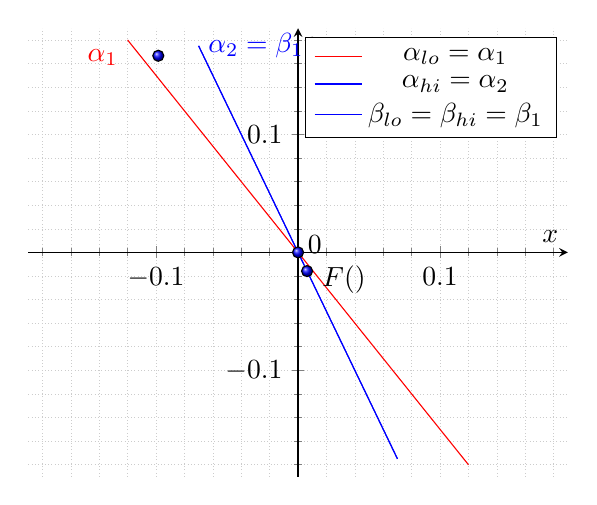
\begin{tikzpicture}
			\begin{axis}[
				axis lines=middle,
				xmin=-0.19,xmax=0.19,ymin=-0.19,ymax=0.19,
				xtick distance=0.1,
				ytick distance=0.1,
				minor tick num = 4,
				xlabel=$x$,
				ylabel=$y$,
				grid=both, 
				grid style={very thin,densely dotted,black!20}]
				\addplot [domain=0.12:-0.12,samples=2, color=red] {x*(-3)/2} node[below left]{$\alpha_1$};
				\addplot [domain=0.07:-0.07,samples=2, color=blue] {x*(-5)/2} node[right]{$\alpha_2 = \beta_1$};
				\addplot [domain=0.07:-0.07,samples=2, color=blue] {x*(-5)/2} node[right]{};
				
				\addlegendentry{$\alpha_{lo} = \alpha_1$}
				\addlegendentry{$\alpha_{hi} = \alpha_2$}		
				\addlegendentry{$\beta_{lo} = \beta_{hi} = \beta_1$}
				
				\addplot [
				only marks,
				mark=ball,
				mark size=2pt,
				point meta=explicit symbolic,
				nodes near coords,
				every node near coord/.append style={yshift=3pt,anchor=west},
				] coordinates {
					(-31/315,1/6) [$\eps$]
					(0,0)    [$\bm{0}$]
				};
			
				\addplot [
			only marks,
			mark=ball,
			mark size=2pt,
			point meta=explicit symbolic,
			nodes near coords,
			every node near coord/.append style={xshift=2pt,yshift=-3pt,anchor=west},
			] coordinates {
				(2/315, -1/63) [$F(\eps)$]
			};
			\end{axis}
		\end{tikzpicture}
	\end{center}
\caption{$\mdp_3$ illustrating case 4.b.i}
\label{fig:2d-plot}
\end{minipage}
\end{figure}
%%
\begin{example}\label{ex:2d}
	We provide an example~$\mdp_3$ with $d=2$,
	where $\eps, F(\eps)$ are vectors incomparable with~$\bm{0}$,
	and $F^2(\eps) = \bm{0}$.
	Here, $\alpha_1(x_1, x_2) = \frac{1}{2}x_1 + \frac{1}{3}x_2$, $\alpha_2(x_1,x_2) = \beta_1(x_1, x_2) = \frac{1}{2}x_1 +\frac{1}{5}x_2$.
	That is, the example fits into the Case~4b.i.
	Let $\eps = (-\frac{31}{315},\frac{1}{6})$. Then, $\alpha_1(\eps) > \alpha_2(\eps)$; we get~$F(\eps) = (\frac{2}{315},-\frac{1}{63})$.
	Further, $\alpha_2(F(\eps)) > \alpha_1(F(\eps))$ and $F^2(\eps) = (0,0)$.
\end{example}



\section{Discussion of Assumptions}\label{sec:discussion}
In this paper, we have made several assumptions for the sake of clarity and simplicity. In this section, we discuss the rationale behind these assumptions, the extent to which these assumptions hold in practice, and the consequences for our protocol when these assumptions hold.

\subsection{Assumptions on the Demand}

There are two simplifying assumptions we make about the demand. First, we assume the demand at any time is relatively small compared to the channel capacities. Second, we take the demand to be constant over time. We elaborate upon both these points below.

\paragraph{Small demands} The assumption that demands are small relative to channel capacities is made precise in \eqref{eq:large_capacity_assumption}. This assumption simplifies two major aspects of our protocol. First, it largely removes congestion from consideration. In \eqref{eq:primal_problem}, there is no constraint ensuring that total flow in both directions stays below capacity--this is always met. Consequently, there is no Lagrange multiplier for congestion and no congestion pricing; only imbalance penalties apply. In contrast, protocols in \cite{sivaraman2020high, varma2021throughput, wang2024fence} include congestion fees due to explicit congestion constraints. Second, the bound \eqref{eq:large_capacity_assumption} ensures that as long as channels remain balanced, the network can always meet demand, no matter how the demand is routed. Since channels can rebalance when necessary, they never drop transactions. This allows prices and flows to adjust as per the equations in \eqref{eq:algorithm}, which makes it easier to prove the protocol's convergence guarantees. This also preserves the key property that a channel's price remains proportional to net money flow through it.

In practice, payment channel networks are used most often for micro-payments, for which on-chain transactions are prohibitively expensive; large transactions typically take place directly on the blockchain. For example, according to \cite{river2023lightning}, the average channel capacity is roughly $0.1$ BTC ($5,000$ BTC distributed over $50,000$ channels), while the average transaction amount is less than $0.0004$ BTC ($44.7k$ satoshis). Thus, the small demand assumption is not too unrealistic. Additionally, the occasional large transaction can be treated as a sequence of smaller transactions by breaking it into packets and executing each packet serially (as done by \cite{sivaraman2020high}).
Lastly, a good path discovery process that favors large capacity channels over small capacity ones can help ensure that the bound in \eqref{eq:large_capacity_assumption} holds.

\paragraph{Constant demands} 
In this work, we assume that any transacting pair of nodes have a steady transaction demand between them (see Section \ref{sec:transaction_requests}). Making this assumption is necessary to obtain the kind of guarantees that we have presented in this paper. Unless the demand is steady, it is unreasonable to expect that the flows converge to a steady value. Weaker assumptions on the demand lead to weaker guarantees. For example, with the more general setting of stochastic, but i.i.d. demand between any two nodes, \cite{varma2021throughput} shows that the channel queue lengths are bounded in expectation. If the demand can be arbitrary, then it is very hard to get any meaningful performance guarantees; \cite{wang2024fence} shows that even for a single bidirectional channel, the competitive ratio is infinite. Indeed, because a PCN is a decentralized system and decisions must be made based on local information alone, it is difficult for the network to find the optimal detailed balance flow at every time step with a time-varying demand.  With a steady demand, the network can discover the optimal flows in a reasonably short time, as our work shows.

We view the constant demand assumption as an approximation for a more general demand process that could be piece-wise constant, stochastic, or both (see simulations in Figure \ref{fig:five_nodes_variable_demand}).
We believe it should be possible to merge ideas from our work and \cite{varma2021throughput} to provide guarantees in a setting with random demands with arbitrary means. We leave this for future work. In addition, our work suggests that a reasonable method of handling stochastic demands is to queue the transaction requests \textit{at the source node} itself. This queuing action should be viewed in conjunction with flow-control. Indeed, a temporarily high unidirectional demand would raise prices for the sender, incentivizing the sender to stop sending the transactions. If the sender queues the transactions, they can send them later when prices drop. This form of queuing does not require any overhaul of the basic PCN infrastructure and is therefore simpler to implement than per-channel queues as suggested by \cite{sivaraman2020high} and \cite{varma2021throughput}.

\subsection{The Incentive of Channels}
The actions of the channels as prescribed by the DEBT control protocol can be summarized as follows. Channels adjust their prices in proportion to the net flow through them. They rebalance themselves whenever necessary and execute any transaction request that has been made of them. We discuss both these aspects below.

\paragraph{On Prices}
In this work, the exclusive role of channel prices is to ensure that the flows through each channel remains balanced. In practice, it would be important to include other components in a channel's price/fee as well: a congestion price  and an incentive price. The congestion price, as suggested by \cite{varma2021throughput}, would depend on the total flow of transactions through the channel, and would incentivize nodes to balance the load over different paths. The incentive price, which is commonly used in practice \cite{river2023lightning}, is necessary to provide channels with an incentive to serve as an intermediary for different channels. In practice, we expect both these components to be smaller than the imbalance price. Consequently, we expect the behavior of our protocol to be similar to our theoretical results even with these additional prices.

A key aspect of our protocol is that channel fees are allowed to be negative. Although the original Lightning network whitepaper \cite{poon2016bitcoin} suggests that negative channel prices may be a good solution to promote rebalancing, the idea of negative prices in not very popular in the literature. To our knowledge, the only prior work with this feature is \cite{varma2021throughput}. Indeed, in papers such as \cite{van2021merchant} and \cite{wang2024fence}, the price function is explicitly modified such that the channel price is never negative. The results of our paper show the benefits of negative prices. For one, in steady state, equal flows in both directions ensure that a channel doesn't loose any money (the other price components mentioned above ensure that the channel will only gain money). More importantly, negative prices are important to ensure that the protocol selectively stifles acyclic flows while allowing circulations to flow. Indeed, in the example of Section \ref{sec:flow_control_example}, the flows between nodes $A$ and $C$ are left on only because the large positive price over one channel is canceled by the corresponding negative price over the other channel, leading to a net zero price.

Lastly, observe that in the DEBT control protocol, the price charged by a channel does not depend on its capacity. This is a natural consequence of the price being the Lagrange multiplier for the net-zero flow constraint, which also does not depend on the channel capacity. In contrast, in many other works, the imbalance price is normalized by the channel capacity \cite{ren2018optimal, lin2020funds, wang2024fence}; this is shown to work well in practice. The rationale for such a price structure is explained well in \cite{wang2024fence}, where this fee is derived with the aim of always maintaining some balance (liquidity) at each end of every channel. This is a reasonable aim if a channel is to never rebalance itself; the experiments of the aforementioned papers are conducted in such a regime. In this work, however, we allow the channels to rebalance themselves a few times in order to settle on a detailed balance flow. This is because our focus is on the long-term steady state performance of the protocol. This difference in perspective also shows up in how the price depends on the channel imbalance. \cite{lin2020funds} and \cite{wang2024fence} advocate for strictly convex prices whereas this work and \cite{varma2021throughput} propose linear prices.

\paragraph{On Rebalancing} 
Recall that the DEBT control protocol ensures that the flows in the network converge to a detailed balance flow, which can be sustained perpetually without any rebalancing. However, during the transient phase (before convergence), channels may have to perform on-chain rebalancing a few times. Since rebalancing is an expensive operation, it is worthwhile discussing methods by which channels can reduce the extent of rebalancing. One option for the channels to reduce the extent of rebalancing is to increase their capacity; however, this comes at the cost of locking in more capital. Each channel can decide for itself the optimum amount of capital to lock in. Another option, which we discuss in Section \ref{sec:five_node}, is for channels to increase the rate $\gamma$ at which they adjust prices. 

Ultimately, whether or not it is beneficial for a channel to rebalance depends on the time-horizon under consideration. Our protocol is based on the assumption that the demand remains steady for a long period of time. If this is indeed the case, it would be worthwhile for a channel to rebalance itself as it can make up this cost through the incentive fees gained from the flow of transactions through it in steady state. If a channel chooses not to rebalance itself, however, there is a risk of being trapped in a deadlock, which is suboptimal for not only the nodes but also the channel.

\section{Conclusion}
This work presents DEBT control: a protocol for payment channel networks that uses source routing and flow control based on channel prices. The protocol is derived by posing a network utility maximization problem and analyzing its dual minimization. It is shown that under steady demands, the protocol guides the network to an optimal, sustainable point. Simulations show its robustness to demand variations. The work demonstrates that simple protocols with strong theoretical guarantees are possible for PCNs and we hope it inspires further theoretical research in this direction.
\bibliography{references}
\end{document}
